\section{Toleranz und Konformität}

Nachdem wir gesehen haben wie wir zwei Hypothesen über die Lage zweier Wahrscheinlich\-keits\-dichte\-ver\-teilungen
verglichen haben, befassen wir uns jetzt mit dem Vergleich von Grenzen, den Toleranzgrenzen, mit einer
Wahrscheinlichkeitsdichteverteilung. Für die Fertigung werden in den Konstruktionszeichnungen zu den Merkmalen
von Bauteilen die Toleranzgrenzen eingetragen, innerhalb derer die Merkmale des Werkstücks liegen müssen. Wie nun
bewertet man nach Fertigstellung des Werkstücks, ob ein Merkmal innerhalb einer Toleranzvorgabe liegt? Ein Merkmal
wird durch einen Messvorgang geprüft. Der Messvorgang liefert ein Ergebnis: Einen Zahlenwert für das Merkmal und
ein Überdeckungsintervall zusammen mit einem Vertrauensniveau. Anstelle von Überdeckungsintervall und Vertrauensniveau
kann auch direkt eine Wahrscheinlichkeitsdichteverteilung angegeben werden, ist aber sehr unüblich in der industriellen
Praxis. Für die Bewertung, ob das gefertigte Werkstück mit der Vorgabe der Konstruktion übereinstimmt, ob es konform ist,
werden Messergebnis und Toleranzvorgabe verglichen.

Als Ergänzung (\textsl{Supplement}) zum \glqq Guide of Uncertainty\grqq ~gibt es das Dokument
\textsl{Evaluation of measurement data - The role of measurement uncertainty in conformity assessment},
das darlegt, wie Konformitätsbewertungen vorzunehmen sind.
\begin{verbatim}
	https://www.bipm.org/documents/20126/2071204/JCGM_106_2012_E.pdf
\end{verbatim}
Dort heißt es in Paragraph 7.1.1
\begin{quote}
	An item conforms to a specified requirement,
	if the true value of its associated property $Y$ lies in the tolerance
	interval. Knowledge of $Y$ is conveyed by a probability density function $p(y|{X_1,\dots,X_J})$
	so that a statement of conformity is always an inference,
	with some probability of being true. Denoting the set of permissible (conforming) values
	$Y$ by $C$, the conformance probability, denoted by $p_\mathrm{c}$, is given by
	\begin{equation}
		p_\mathrm{c} = P(Y \in C | {X_1,\dots,X_J}) = \int\limits_C p(y|{X_1,\dots,X_J}) \mathrm{d}y.
	\end{equation}
\end{quote}
Im Originaldokument werden Sie eine etwas andere Schreibweise für die Bezeichner in der Formel vorfinden.
Hier ist es so aufgeschrieben, wie es zu der Notation innerhalb dieses Vorlesungsskriptes, insbesondere
zu Kapitel \ref{KonzepteinverseProbleme}, passt.
Für die Toleranz wird in der Richtlinie zur Konformitätsbewertung zur Wahrung der Allgemeingültigkeit
eine Menge $C$ angegeben. Falls die Größe $Y$ eine skalarwertige Größe wie bei dem Beispiel, anhand dessen
wir in Kapitel \ref{KonzepteinverseProbleme} das Prinzip der bayesischen Statistik illustriert haben,
so steht $C$ für ein Intervall $C = [T_\mathrm{L}, T_\mathrm{U}]$ im Falle der zweiseitigen
Grenzen, $C = [-\infty, T_\mathrm{U}]$ für den Fall, dass es eine Obergrenze gibt,
$C = [T_\mathrm{L}, \infty]$, dass es eine Untergrenze gibt. Dabei sollen der Index L für \glqq lower
limit\grqq ~und der Index U für \glqq upper limit\grqq ~stehen. Der Bezeichner $T$ ist in der
Normung das üblicherweise für Toleranzgrenzen verwendete Symbol und bedeutet an dieser
Stelle nicht Testgröße! Er unterscheidet sich von den Testgrößen durch seine Indizes.

Die Wahrscheinlichkeit $p_\mathrm{c}$, dass die Beobachtungen ${X_1,\dots,X_J}$ innerhalb des Toleranzintervalls
$C = [T_\mathrm{L}, T_\mathrm{U}]$ liegen, ist
\begin{equation}
	p_\mathrm{c} =  \int\limits_{T_\mathrm{L}}^{T_\mathrm{U}} p(y|{X_1,\dots,X_J}) \mathrm{d}y.
\end{equation}
Für den Fall, dass von einer normalverteilten Stichprobe ausgegangen werden kann und dass eine Einzelgröße
vorliegt, wird auch der Stichprobe ${X_1,\dots,X_J}$ der Schätzer $\bar y$ aus einfacher Mittelwertbildung
gewonnen ($\bar y = \frac{1}{J} \sum\limits_{j=1}^J X_j$) und die Varianz als empirische Varianz $s$ aus
$s^2 = \frac{1}{J-1}\sum\limits_{j=1}^J (X_j - \bar y)^2$ berechnet
und für die Wahrscheinlichkeitsdichte $p$ die Gaußverteilung verwendet
\begin{equation}
	p_\mathrm{c} = \frac{1}{\sqrt{2 \pi} s} \int\limits_{T_\mathrm{L}}^{T_\mathrm{U}}
	e^{-\frac{1}{2}\left(\frac{y - \bar y}{s}\right)^2} \mathrm{d}y .
		\label{eq:Konformitaetswahrscheinlichkeit}
\end{equation}
Die Größe $\frac{y - \bar y}{s}$ ist eine normierte Zufallsgröße. Die Integrationsgrenzen können gleichfalls
normiert werden: $z = \frac{y - \bar y}{s}$, $z_\mathrm{L} = \frac{T_\mathrm{L} - \bar y}{s}$ und
$z_\mathrm{U} = \frac{T_\mathrm{U} - \bar y}{s}$, so dass die Tabellenwerke für die kumulative
standardnormalverteilte Gaußfunktion oder die Bibliotheksfunktion
für die gauß'sche Fehlerfunktion (\textsl{error function}) wie folgt verwendet werden kann:
\begin{equation}
	p_\mathrm{c} = \frac{1}{\sqrt{2 \pi}} \int\limits_{-\infty}^{z_\mathrm{U}}
	e^{-\frac{1}{2} z^2} \mathrm{d}z -
	\frac{1}{\sqrt{2 \pi}} \int\limits_{-\infty}^{z_\mathrm{L}} e^{-\frac{1}{2} z^2} \mathrm{d}z
\end{equation}
d.h.
\begin{equation}
	p_\mathrm{c} = \Phi(z_\mathrm{U}) - \Phi(z_\mathrm{L})
\end{equation}
mit $\Phi(z) = \frac{1}{2} \left(1 + \mathrm{erf}\left(\frac{z}{\sqrt{2}}\right) \right)$. Die Fehlerfunktion ist definiert als
\begin{equation}
	\mathrm{erf}(z)= \frac{2}{\sqrt{\pi}}\int\limits_{0}^{z} \exp (-t^2)\mathrm{d}t
\end{equation}
Die Standardnormalverteilung $\mathcal{N}(\mu=0,\sigma^2=1)$ haben wir mit $\Phi(z)$ bezeichnet. Sie ist wie folgt gegeben:
\begin{equation}
	\Phi(z)= \frac{1}{\sqrt{2\pi}}\int\limits_{-\infty}^{z} \exp (-t^2)\mathrm{d}t
\end{equation}
Mit Hilfe der Toleranzintervalle unterscheidet man zwischen Werten, die mit
Vorgaben beispielsweise der Konstruktion konform sind, und nicht konformen Werten.
Im Toleranzintervall liegen die konformen Werte. Außerhalb des Toleranzintervalls liegen die nicht konformen Werte. Man kann prinzipiell drei Fälle unterscheiden: (a) einseitiges Toleranzintervall mit einer unteren (engl.\ \textsl{lower}) Toleranzgrenze $T_\mathrm{L}$; (b) einseitiges Toleranzintervall mit einer oberen (engl. \textsl{upper}) Toleranzgrenze $T_\mathrm{U}$; (c) zweiseitiges Toleranzintervall mit einer unteren und einer oberen Toleranzgrenze. Die Differenz $T_\mathrm{U} - T_\mathrm{L}$ bezeichnet man als Toleranz.
In Abb.~\ref{fig:Toleranzintervalle} sind diese drei Fälle dargestellt.

\begin{figure}[!htp]
	\begin{center}
		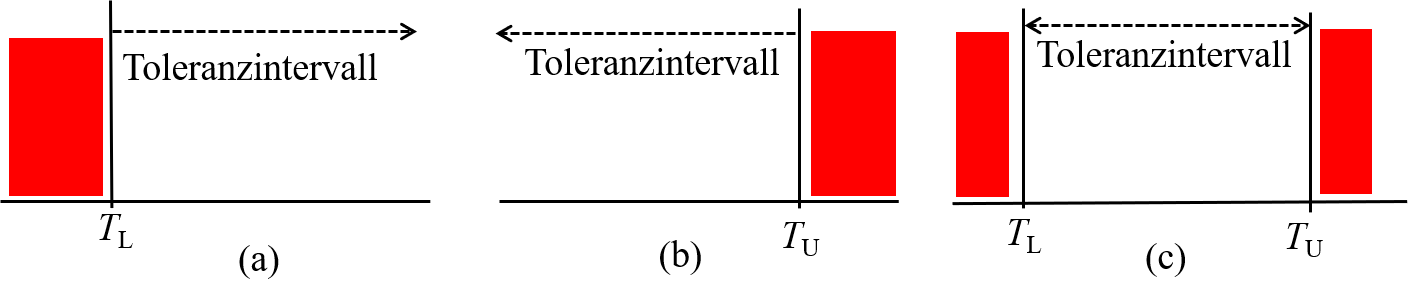
\includegraphics[width=130mm]{05_vorlesung/media/Toleranzintervalle.png}
		\caption{\label{fig:Toleranzintervalle}	Toleranzintervalle} (a) einseitiges Toleranzband mit unterer Toleranzgrenze, (b) einseitiges Toleranzintervall mit oberer Toleranzgrenze (c) zweiseitiges Toleranzintervall
	\end{center}
\end{figure}

\textbf{Beispiel: Geschwindigkeitsmessung} \\
\textsl{Aufgabe:} Berechnen Sie die Konformitätswahrscheinlichkeit $p_\mathrm{c}$ bei einer
Geschwindigkeitsmessung. Die zulässige Geschwindigkeit sei 50~km/h. Der gemessene Wert des Autos liegt bei 52~km/h. Die Geschwindigkeitsmessung sei normalverteilt mit einer Standardunsicherheit $u_y= 1~\mathrm{km/h}$. Berechnen Sie die Konformitätswahrscheinlichkeit
$p_\mathrm{c}$, d.h. die Wahrscheinlichkeit, dass das Auto innerhalb der zugelassenen Geschwindigkeit gefahren ist. \\
\textsl{Lösung:} \\
Geschwindigkeitsbegrenzung: $T_\mathrm{U} = 50~\textrm{km/h}$\\
Gemessener Wert: $\bar y = 52~\textrm{km/h}$ \\
Standardmessunsicherheit: $u_y = 1~\textrm{km/h} $ \\
Die Konformitätswahrscheinlichkeit ergibt sich dann zu:
\[
p_\mathrm{c} = \Phi \left( \frac{T_\mathrm{U}-\bar y}{u_y}\right) = \Phi(-2) = 0.023
\]
Der gemessene Wert von 52~km/h liegt mit einer Wahrscheinlichkeit von 2,3~\% innerhalb des To\-le\-ranz\-inter\-valls, siehe Abb.~\ref{fig:LoesungGeschwindigekeitsmessung}
\begin{figure}[!htp]
	\begin{center}
		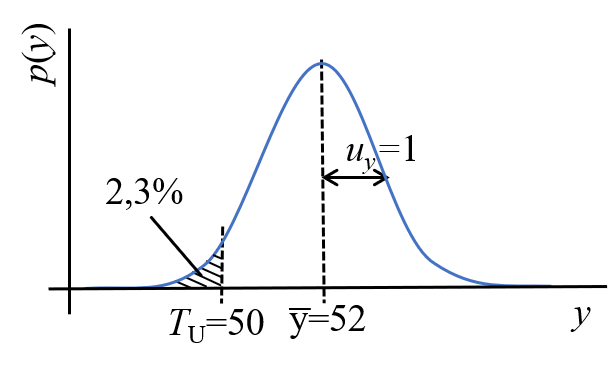
\includegraphics[width=60mm]{05_vorlesung/media/Bsp_Geschwindigkeitsmessung.png}
		\caption{\label{fig:LoesungGeschwindigekeitsmessung} Beispiel: Konformitätswahrscheinlichkeit bei einer Geschwindigkeitsmessung}
	\end{center}
\end{figure}

\section{Konformitätswahrscheinlichkeit und Risiko}
Die wahrscheinlichkeitsbasierte Betrachtung der Konformität ermöglicht die \textsl{Quantifizierung des Risikos einer Fehlbewertung}. Werden beispielsweise bei der Produktion von Widerständen die Widerstandswerte gemessen, so kann ein Toleranzintervall $[T_\mathrm{L}, T_\mathrm{U}]$ definiert werden, in denen die Widerstände noch ok sind und somit auf den Markt gebracht werden. Für den Fall eines einseitigen Toleranzintervalls ist dies in Abb.~\ref{fig:Produktion_Widerstaende} schematisch
dargestellt. Das Risiko einer Fehlbewertung ist dann gegeben durch $1- p_\mathrm{c}$.\\

\begin{figure}[!htp]
	\begin{center}
		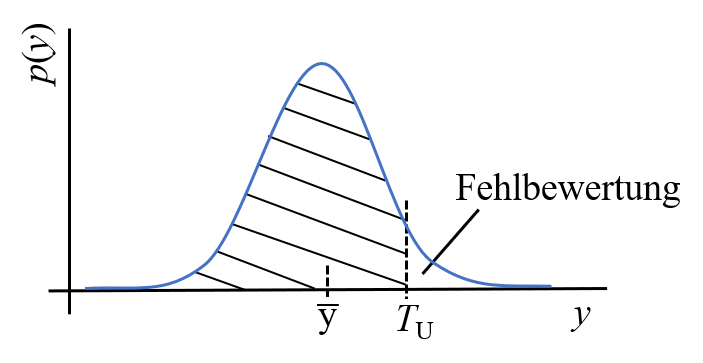
\includegraphics[width=80mm]{05_vorlesung/media/Fehlbewertung.png}
		\caption{\label{fig:Produktion_Widerstaende} Beispiel einer Messung bei einseitigem Toleranzintervall. Der schraffierte Bereich zeigt die Konformitätswahrscheinlichkeit $p_\mathrm{c}$. Das Risiko einer Fehlbewertung ist gegeben durch $1- p_\mathrm{c}$}
	\end{center}
\end{figure}

\begin{quote}
Durch Einführen von Akzeptanzgrenzen und Sicherheitsabständen lässt sich das Risiko einer Fehlbewertung steuern.
\end{quote}

Eine Fehlbewertung kann sowohl eine fälschliche Annahme als auch eine fälschliche Ablehnung sein. Das im folgenden dargestellte Konzept stammt aus dem Dokument \cite{JCGM106}. Es werden -- neben den \textbf{Toleranzgrenzen} $T_\mathrm{L}$ und $T_\mathrm{U}$ -- unterere und oberere \textbf{Akzeptanzgrenzen} $A_\mathrm{L}$,\;$A_\mathrm{U}$ eingeführt.
In folgender Abb.~\ref{fig:Toleranz_Akzeptanzintervall} ist dies schematisch verdeutlicht.
\begin{figure}[!htp]
	\begin{center}
		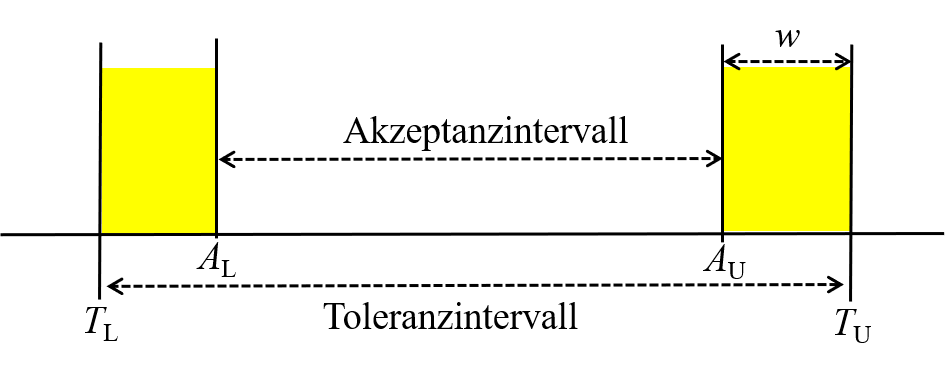
\includegraphics[width=90mm]{05_vorlesung/media/Toleranz_Akzeptanzintervall.png}
		\caption{\label{fig:Toleranz_Akzeptanzintervall} Toleranz- und Akzeptanzintervall. Die Differenz zwischen Toleranzgrenze und Akzeptanzgrenze wird als Sicherheitsabstand / Sicherheitsband bezeichnet.}
	\end{center}
\end{figure}
Die Differenz zwischen Toleranzgrenze und Akzeptanzgrenze definiert einen Längenparameter und wird Sicherheitsabstand $w$ genannt:
\begin{equation}
	w= 	T_\mathrm{U} - A_\mathrm{U}
\end{equation}
In vielen Anwendungen wird dieser Längenparameter als ein Vielfaches der erweiterten Messunsicherheit $U$ angenommen \cite{JCGM106}.
Mit der Wahl der Lage des Akzeptanzintervalls wird das Risiko einer Fehlentscheidung der jeweiligen Situation angemessen ausbalanciert. Es gibt 4 mögliche Resultate einer Konformitätsbewertung. Da wir den tatsächlichen (\glqq wahren\grqq) Wert nicht kennen,
können wir nur auf Grund der Messung entscheiden. Da die Messung jedoch mit einer Messunsicherheit verbunden ist, erhält man bei der Messung eben nicht den wahren Wert.
Es kann dadurch bspw. der Fall eintreten, dass ein Produkt eigentlich innerhalb der zulässigen Toleranzen liegt, jedoch durch die Messung ausgesondert wird. In Abb.~\ref{fig:Resultate_Konformtitaetsbewertung} sind die 4 Resultate einer Konformitätsbewertung dargestellt.

\begin{figure}[!htp]
	\begin{center}
		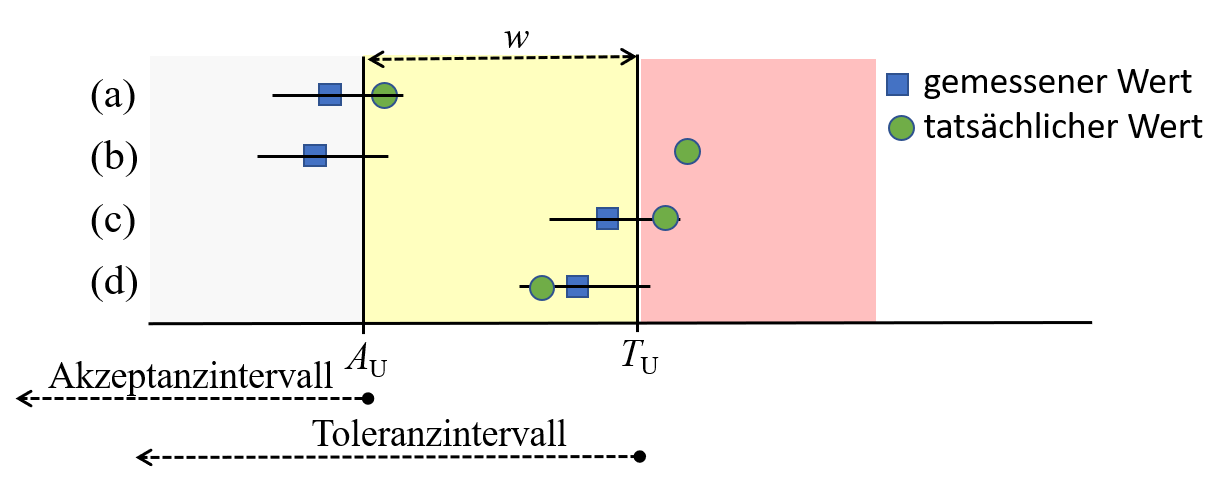
\includegraphics[width=110mm]{05_vorlesung/media/Resultate_der_KFB.png}
		\caption{\label{fig:Resultate_Konformtitaetsbewertung} Resultate der Konformitätsbewertung am Beispiel einseitiger Akzeptanz- und Toleranzgrenzen. (a) Korrekte Annahme, (b) Falsche Annahme -> Konsumentenrisiko, (c) Korrekte Rückweisung, (d) Falsche Rückweisung -> Produzentenrisiko}
	\end{center}
\end{figure}

\begin{itemize}
	\item[(a)] \textbf{Korrekte Annahme / Akzeptanz}: In diesem Fall liegen gemessener und tatsächlicher Wert innerhalb des Toleranzbandes. Dies ist eine richtige Entscheidung.
	\item[(b)] 	\textbf{Falsche Annahme / Akzeptanz}: Der gemessene Wert liegt innerhalb des Akzeptanzbandes, der tatsächliche Wert jedoch außerhalb des Toleranzbandes. Hier wurde bspw. das Produkt angenommen, obwohl es außerhalb der Spezifikationen ist. Dieses Produkt würde auf den Markt gebracht werden, obwohl es nicht innerhalb der Toleranzen ist. Der Konsument hat ein gewisses Risiko, dass das Produkt, das er erhält, nicht konform ist, obwohl es bei einem Inspektionsprozess als konform bewertet wurde. Man spricht hier deshalb auch vom \textbf{Konsumentenrisiko}.
	\item[(c)] 	\textbf{Korrekte Rückweisung}: In diesem Fall liegt der gemessene Wert noch im Toleranzintervall. Das Produkt wird trotzdem verworfen, da es außerhalb des Akzeptanzintervalls liegt. Da der tatsächliche Wert hier außerhalb des Toleranzintervalls liegt, handelt es sich um eine richtige Entscheidung.
	\item[(d)] 	\textbf{Falsche Rückweisung}: Hier liegen gemessener und tatsächlicher Wert außerhalb des Akzeptanzbandes, jedoch noch innerhalb des Toleranzbandes. Das Produkt wird hier, da es außerhalb des Akzeptanzbandes liegt, fälschlicherweise als Ausschuss deklariert. Der Produzent hat stets ein gewisses Risiko, dass ein Produkt durch den Inspektionsprozess fälschlicherweise als Ausschuss deklariert wird. Deshalb spricht man hier vom \textbf{Produzentenrisiko}.
\end{itemize}
Im einfachsten Fall werden die Akzeptanzgrenzen und die Toleranzgrenzen gleichgesetzt. Es werden also Messwerte akzeptiert, die auf der Toleranzgrenze sind. Der (wahre) Wert findet sich somit mit 50\%-iger Wahrscheinlichkeit innerhalb, aber auch genauso
wahrscheinlich außerhalb des zulässigen Toleranzbereichs.
Da in einem solchen Fall eine fifty-fifty-Chance besteht, die
richtige oder falsche Konformitätsentscheidung zu treffen,
wird dieses Verfahren als das \textbf{shared-risk}-Verfahren
bezeichnet (geteiltes Risiko).

\begin{figure}[!htp]
	\begin{center}
		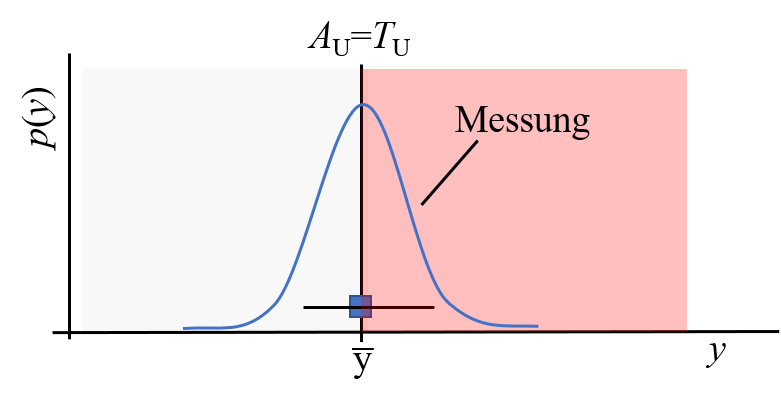
\includegraphics[width=80mm]{05_vorlesung/media/SharedRisk.png}
		\caption{\label{fig:shared_risk} Beispiel für \textsl{shared risk}: Die Akzeptanzgrenze ist gleich der Toleranzgrenze und der Messwert liegt auf dieser Grenze.}
	\end{center}
\end{figure}

Um das Risiko umzuverteilen wird ein Sicherheitsband zwischen Akzeptanz- und Toleranzgrenze eingeführt. Die Länge des Sicherheitsbandes bestimmt das Risiko. Man unterscheidet hier zwischen \textbf{überwachte Annahme} (\textsl{guarded acceptance})
und \textbf{überwachte Ablehnung} (\textsl{guarded rejection}).
Bei der überwachten Annahme wird das Risiko minimiert, fälschlicherweise ein nicht konformes Produkt für gut zu befinden. Hierzu wird die Akzeptanzgrenze tief in das Toleranzintervall hineingelegt, so dass nur solche Messwerte akzeptiert werden, deren zugehörige Unsicherheitsverteilung darauf schließen lassen, den (wahren) Wert mit großer Wahrscheinlichkeit innerhalb des Toleranzbandes zu finden. Der Sicherheitsabstand $w= 	T_\mathrm{U} - A_\mathrm{U}$ ist größer als Null. Die überwachte Annahme spielt bspw. bei Produkten, die man in den Verkehr bringen will, eine Rolle. Man will, dass die Produkte konform mit den Spezifikationen sind.

\begin{figure}[!htp]
	\begin{center}
	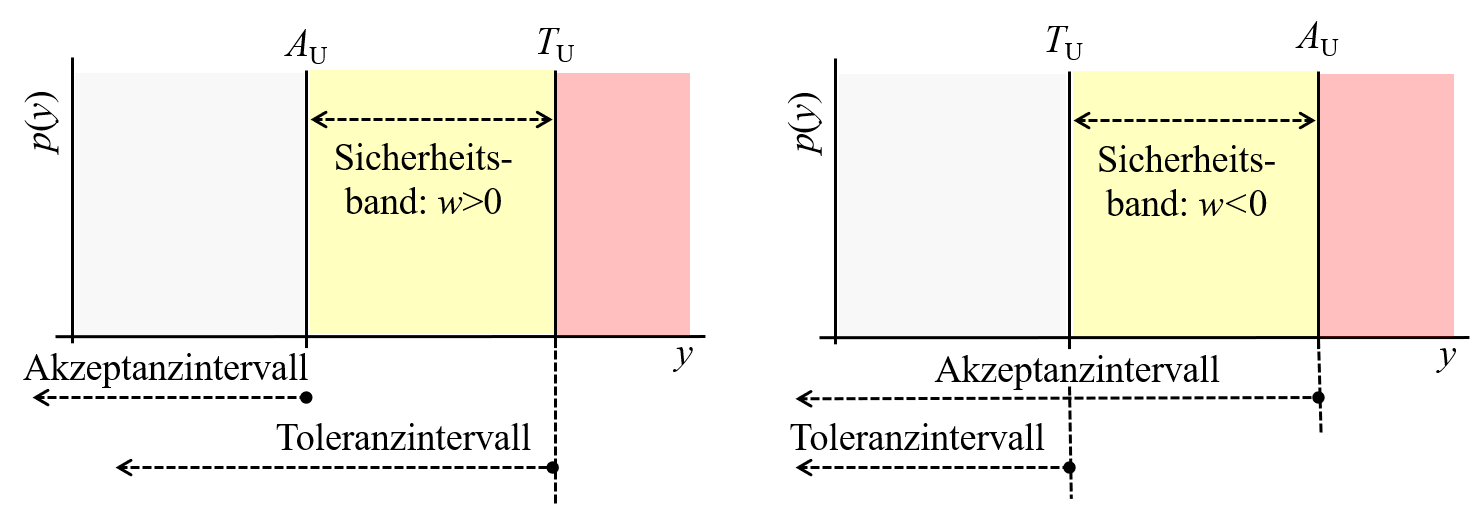
\includegraphics[width=130mm]{05_vorlesung/media/AnnahmeRueckweisungMitToleranz.png}
		\caption{\label{fig:Verteilung_Risiko}} Beispiele für überwachte Annahme (links) und überwachte Rückweisung / Ablehnung (rechts).
	\end{center}
\end{figure}

Bei der überwachten Ablehnung wird das Risiko, dass man zu Unrecht eine Übertretung des Toleranzbandes festgestellt hat, minimiert.
Der Sicherheitsabstand $w= 	T_\mathrm{U} - A_\mathrm{U}$ ist kleiner als Null.
Dies findet bspw. Anwendung bei der Geschwindigkeitsüberwachung im Straßenverkehr und
entspricht der juristischen Entscheidungsregel \glqq in dubio pro reo\grqq ~(lat.\ für \glqq im Zweifel für
den Angeklagten\grqq).

Mit Hilfe der Konformitätswahrscheinlichkeiten $p_\mathrm{c}$ können das \textbf{spezifische Konsumentenrisiko} und das \textbf{spezifische Produzentenrisiko} berechnet werden. Unter dem spezifischen Konsumentenrisiko versteht man die Wahrscheinlichkeit, dass ein einzelner akzeptierter Gegenstand oder ein Produkt angenommen / akzeptiert wird, obwohl er/es nicht konform ist, d.h. nicht innerhalb der Toleranzgrenzen liegt (siehe oben, Fall (b)). Das spezifische Konsumentenrisiko berechnet sich zu $1-p_\mathrm{c}$. Das spezifische Produzentenrisiko ist definiert als die Wahrscheinlichkeit, dass ein einzelner abgelehnter Gegenstand oder ein Produkt konform gewesen wäre. Die Wahrscheinlichkeit, dass ein abgelehnter Gegenstand/Produkt doch konform gewesen wäre, entspricht der Konformitätswahrscheinlichkeit $p_\mathrm{c}$.
Die beiden spezifischen Risiken hängen u.a.\ vom Messwert und Sicherheitsabstand ab. Die
Risiken sind maximal, wenn der Messwert $\bar y = A_\textrm{U}$ ist. Ein positiver Sicherheitsabstand beeinflusst die beiden Risiken in komplementärer Weise. Ein positiver Sicherheitsabstand verkleinert das Konsumentenrisiko und erhöht das Produzentenrisiko.
Ein negativer Sicherheitsabstand verkleinert das Produzentenrisiko und erhöht das Konsumentenrisiko. Für den Fall  \glqq kein Sicherheitsabstand\grqq ~haben wir wieder
den Grenzfall \glqq geteiltes Risiko\grqq.

Neben den spezifischen Risiken werden im \cite{JCGM106} auch die globalen Risiken definiert. Sie geben bspw. die mittlere Wahrscheinlichkeit der Fehleinschätzung basierend auf einem Messprozess an oder die mittlere Wahrscheinlichkeit einer Fehlbewertung über eine große Anzahl durchgeführter Messungen oder die mittlere Wahrscheinlichkeit der Fehlbewertung durch eine zukünftige Messung an. Das globale Risiko ist wichtig für die Planung und hat globale Auswirkungen. Man unterscheidet auch hier zwischen globalem Konsumentenrisiko und globalem Produzentenrisiko.
Gegeben sei das Priorwissen $p_0(y)$ über die Messgröße $Y$ sowie die durchgeführte Messung mit den Messwerten $X_1,\ldots , X_J$. Die durchgeführte Messung wird durch die Wahrscheinlichkeitsdichtefunktion $p(x|y)$ beschrieben. Mit Hilfe des Bayes-Theorems ergibt sich die PDF der Posterior proportional zu $p_0(y)\cdot p(x|y)$. Für das \textbf{globale Konsumentenrisiko} $R_\mathrm{C}$  wird über das Akzeptanzintervall $A$ und über den
Bereich außerhalb des Toleranzintervalls $\tilde C$ integriert:
\begin{equation}
	R_\mathrm{C} =  \int_{\tilde C} \int_{A} \; p_0(y) \cdot p(x|y) \;\mathrm{d}x\; \mathrm{d}y.
	\label{eq:globalesKonsumentenrisiko}
\end{equation}

Für das \textbf{globale Produzentenrisiko} $R_\mathrm{P}$ wird über den Bereich außerhalb des Akzeptanzintervalls $\tilde A$ und über das Toleranzintervall $C$ integriert

\begin{equation}
	R_\mathrm{P} =  \int_{C} \int_{\tilde A} \; p_0(y) \cdot p(x|y) \; \mathrm{d}x\; \mathrm{d}y.
		\label{eq:globalesProduzentenrisiko}
\end{equation}

Ein aus der Richtlinie zur Konformitätsprüfung \cite{JCGM106} entnommenes Beispiel
zeigt sehr anschaulich, wie durch eine dem Produktionsprozess nachgeschaltete
Qualitätsprüfung das Risiko signifikant minimiert, Ausschuss auszuliefern.

Es sollen Widerstände mit einem nominalen Widerstandswert $y_0 = 1500~\Omega$ produziert werden (Vorgabe/ Zielwert). Die Toleranzgrenzen sind wie folgt spezifiziert:
\[
T_\mathrm{L} = 1499.80~\Omega \quad \textrm{und} \quad T_\mathrm{U} = 1500.20~\Omega
\]

Der Erwartungswert des Widerstands sowie die Streuung der Widerstandswerte
durch den Herstellungsprozess sind dem  Menschen nicht bekannt,
aber wir betrachten dies für die Abschätzung der
Risiken, als wüssten wir diese. Wir verwenden als \textsl{wahren} Erwartungswert
den Wert der Zielvorgabe ein und als \textsl{wahre}
Streuung den Wert
\[
\sigma_0 = 0.12~\Omega ,
\]
der daraus gewonnen wurde, dass sich der Hersteller bei Einführung der Produktionslinie
ein ultrapräzises Ohmmeter ausgeliehen hatte, dessen Unsicherheit kleiner ist als
$0.001~\Omega$.
Die Wahrscheinlichkeitsdichteverteilung der produzierten Widerstandswerte
ist der Prior $p_0(y)$ mit
\begin{equation}
p_0(y) \; = \; \frac{1}{\sqrt{2 \pi} \; \sigma_0}
	e^{-\frac{1}{2}\left(\frac{y - y_0}{\sigma_0}\right)^2} \; = \;
 \frac{1}{\sqrt{2 \pi} \cdot 0.12}
	e^{-\frac{1}{2}\left(\frac{y - 1500}{0.12}\right)^2}.
\end{equation}


Wegen der Unsicherheit des Messvorgangs mit dem herstellereigenen Ohmmeter, das er
in seiner Qualitätsprüfung, also bei der Inspektion, einsetzt, ist nicht sichergestellt,
dass wenn ein Widerstand als außerhalb der
Fertigungstoleranz liegend, also außerhalb der Intervalls $[T_\mathrm{L}, T_\mathrm{U}]$
gemessen wird, dass er wirklich außerhalb liegt.
Das in diesem Beispiel in der Qualitätsprüfung verwendete Ohmmeter hat eine
Unsicherheit $u$ von
 \[
\sigma = 0.04~\Omega, \; \mathrm{d.h.}\quad u= 0.04~\Omega \quad \mathrm{bzw.} \quad U(k=2) = 0.08~\Omega
\]
Es kann zum Nachteil des Käufers eines Widerstands passieren,
dass der \textsl{wahre} Wert $x_1$ eines einzelnen Bauteils außerhalb der
Toleranzgrenzen liegt, dass aber das Ohmmeter der Qualitätsprüfung einen Wert misst, der
innerhalb des Akzeptanzintervalls liegt. Abb.~\ref{risikoQS}, \textsl{links}, zeigt ein Beispiel, bei dem der \textsl{wahre} Widerstandswert $y = x_1 = 1500.23 \, \Omega$ beträgt.
Die Wahrscheinlichkeitsdichteverteilung für die Werte, die das Ohmmeter für das
Bauteil mit $x_1 = 1500.23 \, \Omega$ anzeigt, ist
\begin{equation}
p(x | y=x_1) \; = \;  \frac{1}{\sqrt{2 \pi} \; \sigma}
	e^{-\frac{1}{2}\left(\frac{x - x_1}{\sigma}\right)^2} \; = \;
 \frac{1}{\sqrt{2 \pi} \cdot 0.04}
	e^{-\frac{1}{2}\left(\frac{x - 1500.23}{0.04}\right)^2}.
\end{equation}
Das Produkt
\begin{equation}
p(x | y=x_1) \cdot p_0(y=x_1) \; = \; \frac{1}{\sqrt{2 \pi} \; \sigma}
	e^{-\frac{1}{2}\left(\frac{x - x_1}{\sigma}\right)^2}
  \frac{1}{\sqrt{2 \pi} \; \sigma_0} \;
  	e^{-\frac{1}{2}\left(\frac{x_1 - y_0}{\sigma_0}\right)^2}
\end{equation}
mit Einsetzen der Zahlenwerte also
\begin{equation*}
p(x | y=x_1) \cdot p_0(y=x_1)  \; = \;
 \frac{1}{\sqrt{2 \pi} \cdot 0.04}
	e^{-\frac{1}{2}\left(\frac{x - 1500.23}{0.04}\right)^2}
  \frac{1}{\sqrt{2 \pi} \cdot 0.12}
   e^{-\frac{1}{2}\left(\frac{1500.23 - 1500}{0.12}\right)^2}
\end{equation*}
ist als blaue Kurve dargestellt, während der Prior als schwarze Kurve in
dem Diagramm in Abb.~\ref{risikoQS}, \textsl{links}, eingezeichnet ist.
\begin{figure}
\begin{center}
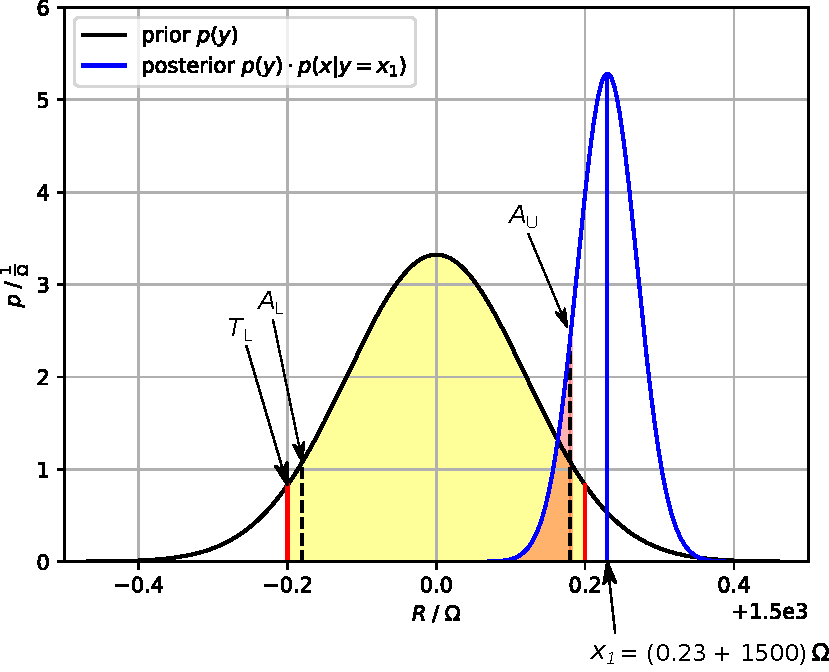
\includegraphics[width=80mm]{05_vorlesung/media/Konsumentenrisiko_x0p03.pdf}
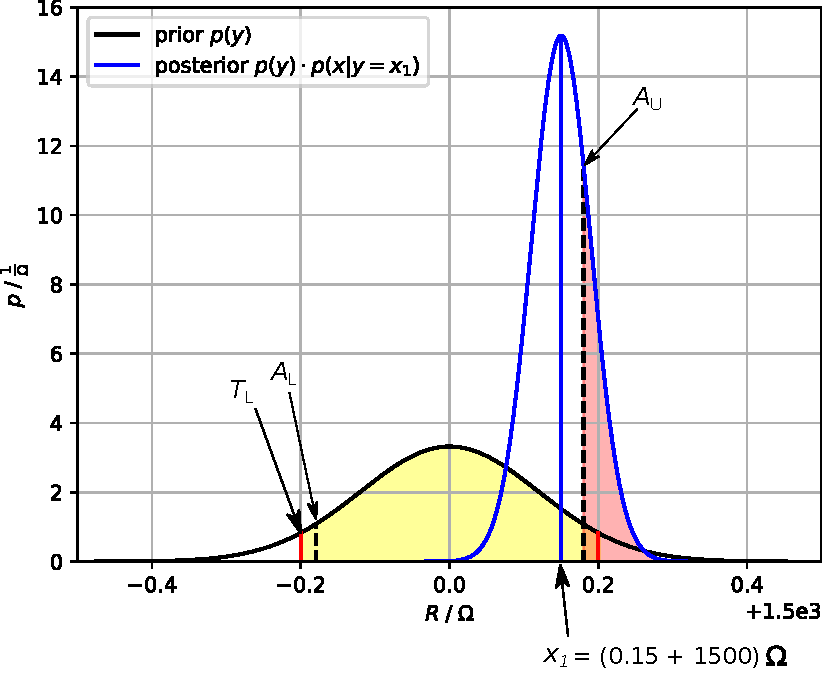
\includegraphics[width=80mm]{05_vorlesung/media/Produzentenrisiko_x0p03.pdf}
\caption{Veranschaulichung zur Berechnung der globalen Risiken, \textsl{links:}
des Konsumenten bzw.\ Käufers, (\textsl{rechts}) des Produzenten bzw.\
Herstellers}
\label{risikoQS}
\end{center}
\end{figure}

Es kann zum Nachteil des Herstellers passieren, dass der \textsl{wahre} Wert
eines einzelnen Bauteils $x_1$ innerhalb der
Toleranzgrenzen - sogar innerhalb des Akzeptanzintervalls - liegt,
dass aber das Ohmmeter der Qualitätsprüfung einen Wert misst, der
außerhalb des Akzeptanzintervalls liegt. Abb.~\ref{risikoQS}, \textsl{rechts}, zeigt ein Beispiel, bei dem der \textsl{wahre} Widerstandswert $y = x_1 = 1500.15 \, \Omega$ beträgt.
Hier sind das Produkt
\begin{equation*}
p(x | y=x_1) \cdot p_0(y=x_1) \; = \;
 \frac{1}{\sqrt{2 \pi} \cdot 0.04}
	e^{-\frac{1}{2}\left(\frac{x - 1500.15}{0.04}\right)^2}
  \frac{1}{\sqrt{2 \pi} \cdot 0.12}
   e^{-\frac{1}{2}\left(\frac{1500.15 - 1500}{0.12}\right)^2}
\end{equation*}
wieder als blaue Kurve und der Prior als schwarze Kurve zu sehen.

Die roten Flächen unter den Kurven der beiden Diagramme in Abb.~\ref{risikoQS}
zeigen jeweils die Wahrscheinlichkeit dafür, dass im Falle \textsl{links} mit
$y = x_1 = 1500.23 \, \Omega$ der schlechte Widerstand mit einen Wert innerhalb des
Akzeptanzintervalls gemessen wird, folglich als gut verkauft wird, und dass im Falle \textsl{rechts} mit
$y = x_1 = 1500.15 \, \Omega$ der gute Widerstand mit einen Wert außerhalb des
Akzeptanzintervalls gemessen wird, folglich als schlecht verworfen wird.

Berechnet man für alle Werte $x_1$, die außerhalb des Toleranzintervalls die roten
Flächen der Teile solcher Produktkurven $p(x | y=x_1) \cdot p_0(y=x_1)$ d.h.\ integriert
man $x$ über diesen Bereich wie im linken Diagramm,
 um die Wahrscheinlichkeiten, dass schlechte Widerstände als gut
gemessen und somit verkauft werden, zu bestimmen und integriert dann noch
über alle diese Werte $x_1$, so erhält man die Wahrscheinlichkeit des Risikos, dass
der Käufer / Konsument  trotz Qualitätsprüfung Ausschussware erhält. Diese
Wahrscheinlichkeit heißt \textbf{globales Konsumentenrisiko}.

Berechnet man für alle Werte $x_1$, die innerhalb des Toleranzintervalls die roten
Flächen der Teile solcher Produktkurven $p(x | y=x_1) \cdot p_0(y=x_1)$ d.h.\ integriert
man $x$ über diesen Bereich wie im rechten Diagramm,
 um die Wahrscheinlichkeiten, dass gute Widerstände als schlecht
gemessen und somit als Ausschuss verworfen werden, zu bestimmen und integriert dann noch
über alle diese Werte $x_1$, so erhält man die Wahrscheinlichkeit des Herstellers
trotz Qualitätsprüfung gute Ware vernichtet. Diese
Wahrscheinlichkeit heißt \textbf{globales Produzentenrisiko}.

Dieses Beispiel zeigt, dass der Aufwand lohnt, in einen Qualitätssicherungsprozess zu investieren.

Die Konformitätswahrscheinlichkeit $p_\mathrm{c}$, Gl.~(\ref{eq:Konformitaetswahrscheinlichkeit}), liegt in diesem Beispiel bei
\[
	p_\mathrm{c} = \frac{1}{\sqrt{2 \pi} s} \int\limits_{T_\mathrm{L}}^{T_\mathrm{U}}
e^{-\frac{1}{2}\left(\frac{y - \bar y}{s}\right)^2} \mathrm{d}y  =
\frac{1}{\sqrt{2 \pi} \cdot 0.12} \int\limits_{T_\mathrm{L}=1499.80}^{T_\mathrm{U}=1500.20}
e^{-\frac{1}{2}\left(\frac{y - 1500}{0.12}\right)^2} \mathrm{d}y  \approx 0.905
\]
was bedeutet, dass im Rahmen des Produktionsprozesses etwa 90\% der Widerstände konform sind,
jedoch 10\% der Widerstände, die auf den Markt gebracht würden, nicht konform wären. Das Konsumentenrisiko
liegt somit bei 10\% Ausschussware.

Die Akzeptanzgrenzen werden innerhalb des Toleranzintervalls gewählt, um das
Konsumentenrisiko zu reduzieren:
\[
A_\mathrm{L} = 1499.82~\Omega \quad \textrm{und} \quad A_\mathrm{U} = 1500.18~\Omega
\]
Das Sicherheitsband beträgt $w = (1500.20-1500.18)~\Omega = 0.02~\Omega = 0.25 U$

Im Vergleich zu den $10 \, \%$ Ausschuss liefert
\begin{itemize}
\item das globale Konsumentenrisiko, Gl.(\ref{eq:globalesKonsumentenrisiko}),
\begin{equation}
	R_\mathrm{C} =  \int_{\tilde C} \int_{A} \; p_0(y) \; p(x|y) \;\mathrm{d}x\; \mathrm{d}y
	\label{eq:globalesKonsumentenrisiko_Aufg}
\end{equation}
d.h.
$$
R_\mathrm{C} =  \int\limits_{-\infty}^{T_\mathrm{L}} \, \mathrm{d}y\; p_0(y) \;
 \int\limits_{A_\mathrm{L}}^{A_\mathrm{U}} \mathrm{d}x \; p(x|y) \; + \;
 \int\limits_{T_\mathrm{U}}^{\infty} \, \mathrm{d}y\; p_0(y) \;
  \int\limits_{A_\mathrm{L}}^{A_\mathrm{U}} \mathrm{d}x \; p(x|y)
$$
mit
\begin{equation}
	p(x|y) =\frac{1}{\sqrt{2 \pi} \sigma}
	e^{-\frac{1}{2}\left(\frac{x - y}{\sigma}\right)^2} =
	\frac{1}{\sqrt{2 \pi} \cdot 0.04}
		e^{-\frac{1}{2}\left(\frac{x - y}{0.04}\right)^2}
\end{equation}
und nach Einsetzen der Zahlenwerte
$$
 R_\mathrm{C} = \int\limits_{-\infty}^{T_\mathrm{L}} \, \mathrm{d}y\;
 \frac{1}{\sqrt{2 \pi} \cdot 0.12}
 e^{-\frac{1}{2}\left(\frac{y - 1500}{0.12}\right)^2}
 \int\limits_{A_\mathrm{L}}^{A_\mathrm{U}} \mathrm{d}x \;
 \frac{1}{\sqrt{2 \pi} \cdot 0.04}
   e^{-\frac{1}{2}\left(\frac{x - y}{0.04}\right)^2}
$$
$$
   \; + \;
   \int\limits_{T_\mathrm{U}}^{\infty} \, \mathrm{d}y\;
  \frac{1}{\sqrt{2 \pi} \cdot 0.12}
  e^{-\frac{1}{2}\left(\frac{y - 1500}{0.12}\right)^2}
  \int\limits_{A_\mathrm{L}}^{A_\mathrm{U}} \mathrm{d}x \;
  \frac{1}{\sqrt{2 \pi} \cdot 0.04}
    e^{-\frac{1}{2}\left(\frac{x - y}{0.04}\right)^2}
  \; \approx \; 1~\%
$$
\item Das globale Produzentenrisiko berechnet sich mit Gl.(\ref{eq:globalesProduzentenrisiko}) zu
\begin{equation}
	R_\mathrm{P} =  \int_{C} \int_{\tilde A} \; p_0(y) \; p(x|y) \; \mathrm{d}x\; \mathrm{d}y
  \label{eq:globalesProduzentenrisiko_Aufg}
\end{equation}
$$
	=  \int\limits_{T_\mathrm{L}}^{T_\mathrm{U}} \, \mathrm{d}y\; p_0(y) \;
 \left(\int\limits_{-\infty}^{A_\mathrm{L}} \mathrm{d}x \; p(x|y)
 + \int\limits_{A_\mathrm{U}}^{\infty} \mathrm{d}x \; p(x|y) \right)  \approx 7~\%
$$
\end{itemize}
Die beiden Integrale Gl.~(\ref{eq:globalesKonsumentenrisiko_Aufg})
und Gl.~(\ref{eq:globalesProduzentenrisiko_Aufg}) werden numerisch gelöst,
siehe auch \cite{JCGM106}.

Die Wahrscheinlichkeitsaussagen liefen Größenordnungen, über die man sich vorstellen kann,
dass beispielsweise von 100 produzierten Widerständen um die 90 Bauteile im Produktionsprozess 90 innerhalb der Toleranzen liegen und damit in etwa so 10 Bauteile Ausschuss sind. Wenn es
einen Inspektionsprozess zur Qualitätssicherung gibt, so kann es passieren, dass von 90 guten, innerhalb der Toleranz liegenden Bauteilen vielleicht um die 7 fälschlicherweise als nicht konform ausgemustert. Umgekehrt kann es passieren, dass von 10 Ausschussteilen eines fälschlicherweise akzeptiert und somit an einen Kunden verkauft wird.

Dieses Beispiel veranschaulicht, dass sie eine Qualitätsprüfung lohnt:
Durch sie wurde das Risiko des Käufers,
Ausschussware geliefert zu bekommen, in diesem Beispiel
von knapp 10\% auf ungefähr 1\% reduziert, und damit das
Problem von Reklamation und Regressansprüchen signifikant reduziert.

Matlab/Octave-Code zur numerischen Berechnung des Konsumenten- und Produktionsrisikos:

\begin{lstlisting}[style=Matlab]
  function konform_example_R()
  step = 0.0002;
  perc = '%';

  gaussian = @(x, mu, sigma) exp(-0.5*((x - mu) / sigma).^2) / (sigma * sqrt(2*pi));

% ----
  y0 = 1500;
  s0 = 0.12;
  T_L = 1499.80;
  T_U = 1500.20;
  A_L = 1499.82;
  A_U = 1500.18;
  mininf = T_L - 3*s0;
  maxinf = T_U + 3*s0;

  y = [A_L:step:A_U];
  prior = step * gaussian(y, y0, s0);
  p_c = sum(prior);
  printf('spezifisches Konsumentenrisiko bzgl A ..................: %3.0f %c\n', ...
    100 - 100*p_c, perc);

  y = [T_L:step:T_U];
  prior = step * gaussian(y, y0, s0);
  p_c = sum(prior);
  printf('spezifisches Konsumentenrisiko bzgl T Gl (21) in JCGM106: %3.0f %c\n', ...
    100 - 100*p_c, perc);

% inspection device - instrument uncertainty
  s_insp = 0.04;

% ------
% global producer risk:
  x_L = [mininf:step:A_L]'; %'
  x_U = [A_U:step:maxinf]'; %'

  n_y = length(y);
  n_xL = length(x_L);
  n_xU = length(x_U);

  px_giveny_L = step * gaussian(x_L * ones(1,n_y), ones(n_xL,1) * y, s_insp);
  px_giveny_U = step * gaussian(x_U * ones(1,n_y), ones(n_xU,1) * y, s_insp);

  posterior_L = (ones(n_xL,1)*prior) .* px_giveny_L;
  posterior_U = (ones(n_xU,1)*prior) .* px_giveny_U;
  R_p = sum(posterior_L(:)) + sum(posterior_U(:));
  printf('globales Produzentenrisiko: %3.0f %c\n', 100*R_p, perc);

%-------
% global consumer risk

  x = [A_L:step:A_U]'; %'
  y_L = [mininf:step:T_L];
  y_U = [T_U:step:maxinf];

  n_x = length(x);
  n_yL = length(y_L);
  n_yU = length(y_U);
  prior_L = step * ones(n_x,1) * gaussian(y_L, y0, s0);
  prior_U = step * ones(n_x,1) * gaussian(y_U, y0, s0);
  px_giveny_L = step * gaussian(x * ones(1,n_yL), ones(n_x,1) * y_L, s_insp);
  px_giveny_U = step * gaussian(x * ones(1,n_yU), ones(n_x,1) * y_U, s_insp);
  posterior_L = prior_L .* px_giveny_L;
  posterior_U = prior_U .* px_giveny_U;
  R_c = sum(posterior_L(:)) + sum(posterior_U(:));
  printf('globales Konsumentenrisiko: %3.0f %c\n', 100*R_c, perc);
end

\end{lstlisting}
